\documentclass[conference,compsoc]{IEEEtran}
\usepackage{graphicx}
\usepackage[spanish,es-tabla]{babel}
\usepackage[T1]{fontenc}
\usepackage{fontspec}
\usepackage{listings}
\usepackage{svg}
\usepackage{anyfontsize}
\usepackage{hyperref}
\graphicspath{ {figures/} }
\hypersetup{colorlinks = false}
\lstset{language=SQL,morekeywords={PREFIX,java,rdf,rdfs,url,@prefix}}
\newcommand{\rdf}{\textit{RDF}\ }
\newcommand{\spql}{\texttt{SPARQL}\ }

\begin{document}

\title{SUGERENCIAS PARA LA CONSTRUCCIÓN DE CONSULTAS SPARQL, UNA ALTERNATIVA OPEN SOURCE\\ \ \\PROPUESTA}

\author{
    \IEEEauthorblockN{Carlos Andrés Ponce Godoy}
    \IEEEauthorblockA{\textit{Departamento de Informática} \\
    \textit{Universidad Técnica Federico Santa María}\\
    Valparaíso, Chile\\
    carlos.ponce@sansano.usm.cl}
}

\maketitle

\IEEEpubidadjcol

\begin{abstract}
    \spql es el lenguaje utilizado para realizar consultas a las bases de datos orientadas
    a grafos, las cuales, en el contexto de la web semántica, almacenan los datos en forma
    de tríos \textit{sujeto - predicado - objeto} a través del formato \rdf. Sin embargo,
    para un usuario con pocos conocimientos sobre la web semántica, escribir una consulta
    \spql es una tarea que implica un alto esfuerzo cognitivo. Existen herramientas como
    \textit{RDF Explorer} que permiten construir consultas de forma interactiva. Pero no es
    suficiente, puesto que aún le exigimos al usuario conocer el esquema y los contenidos
    de la base de datos con la que trabajamos. Para esto podemos recomendar al usuario que entidades
    puede consultar. En este trabajo buscamos realizar mejores al rendimiento del proyecto
    \textit{SPARQLforHumans} el cual puede generar recomendaciones a consultas \spql incompletas
    y puede ser integrado con la interfaz \textit{RDF Explorer}.
\end{abstract}

\begin{IEEEkeywords}
    SPARQL, Web Semántica, RDF
\end{IEEEkeywords}

\IEEEpeerreviewmaketitle

\section{Definición del problema}

La web semántica es un conjunto de extensiones para la \textit{World Wide Web},
desarrolladas por el \textit{World Wide Web Consortium (W3C)} para permitir que
la información disponible en la internet pueda ser procesada por máquinas \cite{berners2001semantic}.

Para lograr esto, la web semántica propone agregar a la información ya existente
metadatos semánticos para que estos puedan ser procesados por agentes inteligentes,
los cuales obtendrán esta información sin operadores humanos. Estos metadatos pueden
ser descritos utilizando múltiples estándares existentes, uno de ellos es el
\textit{Resource Description Framework (RDF)}, el cual define una estructura para
definir relaciones entre entidades \cite{world2014rdf}.

Estas relaciones se describen a través de un trio \textit{sujeto - predicado - objeto},
en el cual, cada uno de los elementos está representado por un \textit{Uniform Resource Identifier (URI)}.
Estas relaciones descritas en \rdf pueden ser visualizadas a través de grafos dirigidos como
el que se encuentra en la figura \ref{fig:rdf-graph1}

\begin{figure}%[h]
    \centering
    \includesvg[width=\linewidth]{rdf-graph.svg}
    \caption{Un grafo \rdf con dos nodos \textit{Subject} y \textit{Object} conectados a través de
    la relación \textit{Predicate}.}
    \label{fig:rdf-graph1}
\end{figure}

Un conjunto de múltiples tríos que describen múltiples relaciones para una gran cantidad
de entidades se almacena en una \textit{Triplestore}, la cual consiste en una base de datos
diseñada para responder a consultas al estilo \textit{sujeto - predicado - objeto} del 
formato \rdf \cite{rusher2001triple}.

El lenguaje utilizado para obtener datos e información desde una \textit{Triplestore} es
\spql y su nombre corresponde a un acrónimo recursivo, el cual significa \textit{SPARQL
Protocol and RDF Query Language} \cite{world2013sparql}.

El ejemplo más básico de una consulta \spql es el que utiliza las sentencias \texttt{SELECT}
y \texttt{WHERE}. Primero, definimos nuestro conjunto de datos en el bloque de código \ref{lst:basic-rdf}.

\begin{figure*}
    \begin{lstlisting}[captionpos=b, caption=Datos en formato \rdf., label=lst:basic-rdf, basicstyle=\ttfamily, frame=single]
@prefix exbook: <http://example.org/book>
@prefix purl: <http://purl.org/dc/elements/1.1>

exbook:book1 purl:title "SPARQL Tutorial" .
     \end{lstlisting}
\end{figure*}

Luego, realizamos la consulta con las siguientes sentencias, como se puede observar en
el segmento de código \ref{lst:basic-sparql}.

\begin{figure*}
    \begin{lstlisting}[captionpos=b, caption=Consulta SPARQL basica., label=lst:basic-sparql, basicstyle=\ttfamily, frame=single]
PREFIX exbook: <http://example.org/book>
PREFIX purl: <http://purl.org/dc/elements/1.1>
SELECT ?title
WHERE {
    exbook:book1 purl:title ?title .
}
     \end{lstlisting}
\end{figure*}

En base a nuestro conjunto de datos disponible, solo existe una
solución al patrón del grafo descrito en la consulta, el resultado es la tabla \ref{tab:basic-result}.

\begin{table}[h]
    \label{tab:basic-result}
    \caption{Resultado de una consulta SPARQL básica}
    \centering
    \resizebox{0.55\linewidth}{!}{\begin{tabular}{|c|}
    \hline
    title               \\ \hline
    ``SPARQL Tutorial"   \\ \hline
    \end{tabular}}
\end{table}

En base a todo lo anterior, podemos notar que escribir este tipo de consultas no es
sencillo e implica un esfuerzo cognitivo importante. Actualmente, si una persona
quisiera realizar una consulta a una \textit{Triplestore} o base de datos con soporte \spql, necesitará
conocer dos cosas, la sintaxis de \spql y la estructura de la base de datos que estamos
consultando.

Para apoyar a los nuevos usuarios a satisfacer estas dos necesidades, se han desarrollado
herramientas y plataformas que facilitan la construcción de consultas y la exploración
de las entidades en las bases de datos \rdf como por ejemplo, \textit{RDFExplorer}
\cite{vargas2019rdf}, \textit{Tabulator} \cite{berners2006tabulator} , \textit{Explorator}
\cite{araujo2009experimenting}, \textit{DBpedia Atlas} \cite{valsecchi2015dbpedia},
\textit{RDF Visualizer} \cite{sayers2004node}, \textit{SPARQL Assist}
\cite{mccarthy2012sparql} o \textit{YASGUI} \cite{rietveld2017yasgui}.

Estas herramientas nos facilitan la tarea de explorar los contenidos de la base de datos \rdf
y además nos permiten construir consultas \spql de forma interactiva. Para nuestro trabajo,
hemos decidido trabajar con la plataforma \textit{RDFExplorer} (figura \ref{fig:rdfexplorer}) debido a las siguientes
características que presenta:

\begin{itemize}
    \item Facilidad de usó.
    \item Construcción interactiva de consultas \spql.
    \item Navegación de entidades en la base de datos.
    \item Generación de resultados parciales.
    \item Código fuente disponible y abierto \cite{vargas2019rdfrepo}.
\end{itemize}

\begin{figure*}
    \centering
    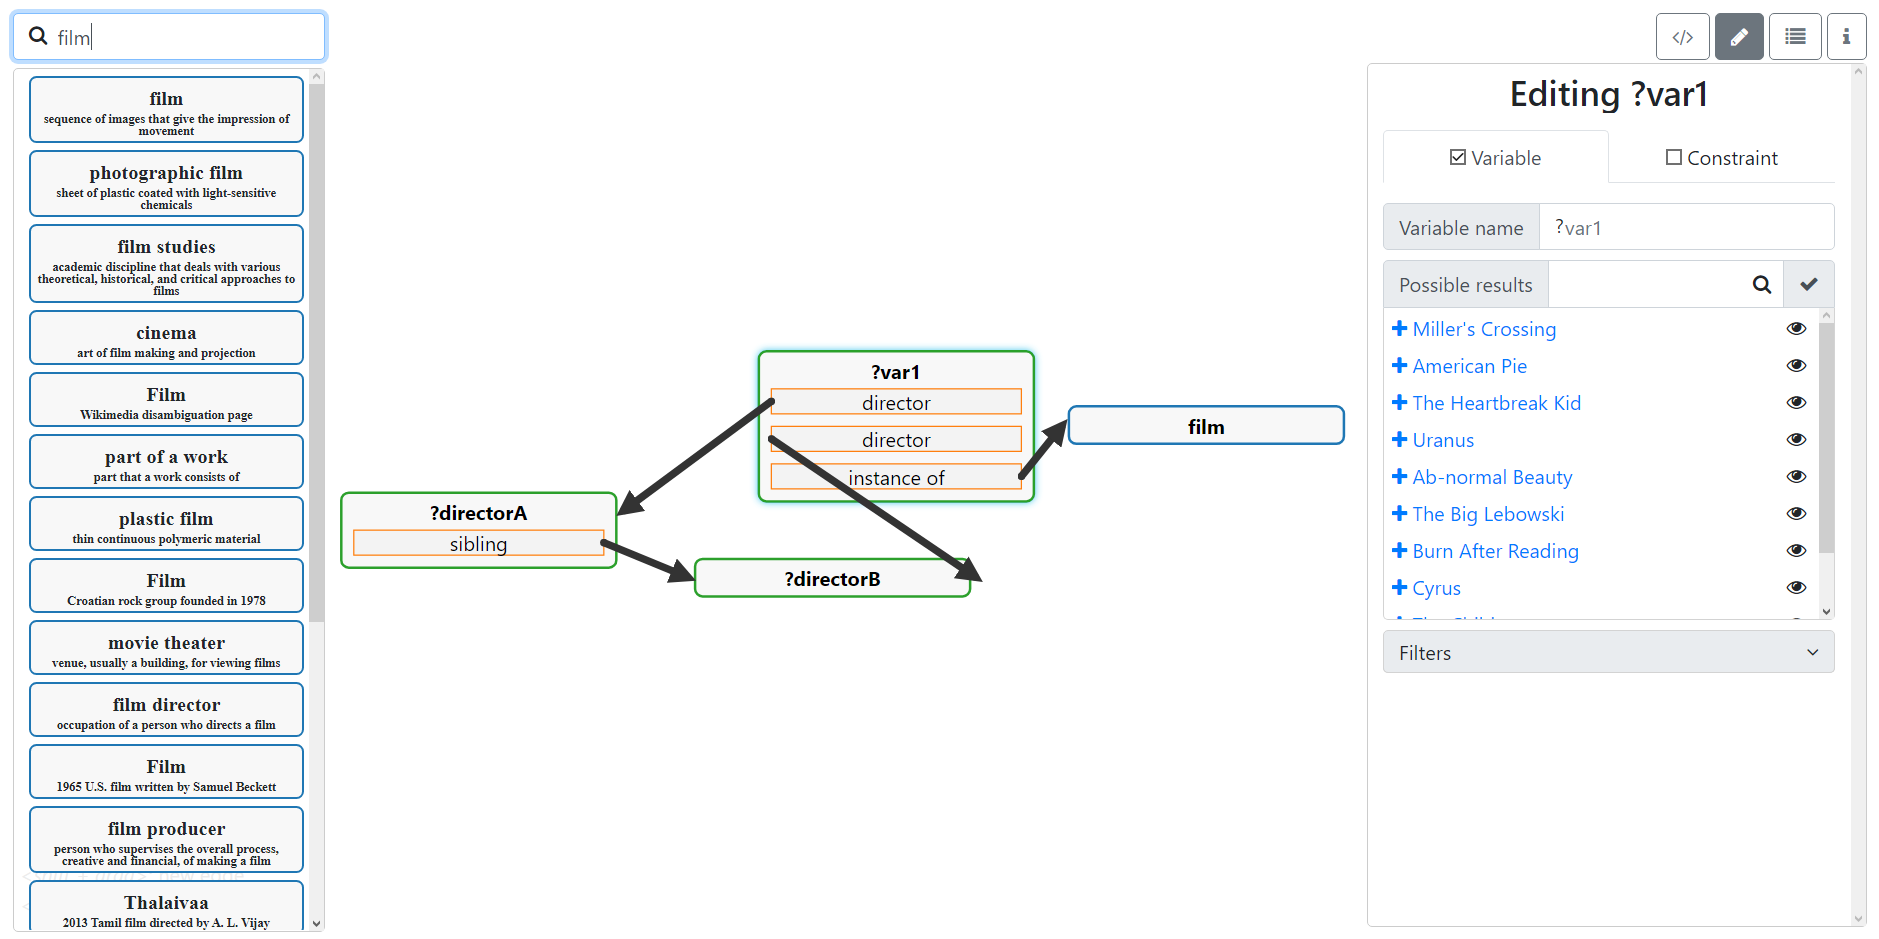
\includegraphics[width=\linewidth]{rdfexplorer.png}
    \caption{RDF Explorer, construcción de una consulta \spql que obtiene las películas dirigidas
    por hermanos, a la derecha, un conjunto de posibles resultados.}
    \label{fig:rdfexplorer}
\end{figure*}

Sin embargo, aun cuando utilizamos herramientas como \textit{RDFExplorer}, debemos tener
algún grado de conocimiento sobre las propiedades de las entidades disponibles
en la base de datos, los cuales no tenemos cuando somos nuevos usuarios.

Una forma de apoyar a estos usuarios en la tarea de descubrir las propiedades disponibles
en nuestra \textit{Triplestore} es generar recomendaciones o sugerencias sobre los \textit{predicados}
disponible para una determinada entidad, esto es similar a lo realizado por herramientas de autocompletado
al escribir documentos o lo que es más cercano al campo de la programación y la informática, el
autocompletado de código realizado por entornos de desarrollo integrados \cite{bruch2009learning}.

Actualmente, existen soluciones y herramientas que nos permiten obtener recomendaciones en base a 
consultas \spql incompletas como \textit{Gosparqled} \cite{campinas2014live}, \textit{LinkedWiki editor}
\cite{rafes2018designing}, \textit{SPARKLIS} \cite{ferre2017sparklis}, \textit{SPACE} \cite{kramer2013space}
y \textit{SPARQLforHumans} \cite{parra2020autocompletion}.

De las anteriores alternativas, la única que actualmente se encuentra integrada con \textit{RDFExplorer}
es \textit{SPARQLforHumans}. Sin embargo, esta solución tiene un problema fundamental, su implementación
se ha realizado utilizando el lenguaje de programación $C\#$ y el framework \texttt{.NET} en el sistema
operativo \textit{Windows} lo cual limita los entornos de ejecución disponibles en los que puede ser utilizado,
debido a que, además, depende directamente de las bibliotecas \textit{DLL} del proyecto \textit{Apache Lucene}
\cite{bialecki2012apache}.

% si bien actualmente los componentes del framework se encuentran bajo las licencias MIT o Apache 2, 
% la propiedad sigue perteneciendo a la empresa Microsoft, la cual, es conocida por su compleja historia
% con la comunidad de código abierto.

En base a todo lo expuesto anteriormente, con este trabajo buscamos replicar la funcionalidad obtenida por
el proyecto \textit{SPARQLforHumans} pero con una restricción importante, los componentes de nuestra arquitectura
solo pueden corresponder a software gratuito y de código abierto. Además, buscamos realizar las siguientes mejoras
al rendimiento global del sistema:

\begin{itemize}
    \item Reducir el tiempo de procesamiento para los volcados de la base de datos de Wikipedia.
    \item Reducir el tiempo necesario para generar una recomendación a una consulta \spql incompleta.
\end{itemize}

\section{Objetivos}

    \subsection{Objetivo general}

Diseñar e implementar mejoras al rendimiento de la arquitectura propuesta por el proyecto
\textit{SPARQLforHumans}, utilizando exclusivamente componentes de código abierto.

    \subsection{Objetivos específicos}

\begin{itemize}
    \item Diseñar el mecanismo de recomendación para las entidades de una consulta.
    \item Diseñar la arquitectura del sistema utilizando solamente componentes de código abierto.
    \item Implementar la arquitectura propuesta.
    \item Evaluar el rendimiento de la solución implementada.
\end{itemize}

\section{Discusión bibliográfica preliminar}

Para abordar nuestro problema primero debemos aclarar algunos conceptos que han sido
mencionados en las secciones anteriores de manera más formal, tales como la web semántica, SPARQL, RDF y el
contexto en el que estos se utilizan. Para esto, nos apoyaremos en las siguientes definiciones.

    \subsection{La web semántica}

La red informática mundial, \textit{World Wide Web} o simplemente \textit{Web} es el sistema de información público más importante
desarrollado en los últimos 30 años, el cual permite la transmisión de documentos electrónicos identificados
por \texttt{URIs} \textit{(Uniform Resource Identifiers)}, los cuales pueden estar enlazados a otros documentos
a través de \texttt{hipertexto} y que se encuentran disponibles utilizando servicios de la internet.

La \textit{World Wide Web} fue diseñada como un espacio para la información con el objetivo de no solo ser
útil para las comunicaciones entre humanos, sino que también un lugar donde las máquinas podrían ayudar y participar.
Sin embargo, uno de los principales problemas de la \textit{Web} es que la mayor parte de su contenido ha sido
diseñado para ser consumido por humanos, lo que implica que para las máquinas y el software no es fácil acceder 
e interpretar el contenido disponible, incluso si este proviene de una base de datos estructurada a través de
columnas claras y tipificadas. La web semántica busca desarrollar herramientas,
lenguajes, protocolos y estándares que permitan, tanto a maquinas como humanos, procesar toda la información disponible en la
\textit{Web}. En base a esto, podemos definir a la web semántica como la idea de generar
una red de datos en la \textit{Web}, hasta cierto punto, una base de datos global. \cite{berners1998semantic}

    \subsection{Arquitectura de la web semántica}

La web semántica está construida en base a múltiples bloques, los cuales representan estándares y lenguajes
utilizados para lograr determinadas funcionalidades descritas en su arquitectura \cite{harth2011semantic}, una representación gráfica
de esta arquitectura en bloques se puede observar en la figura \ref{fig:semantic-web-arq}, la cual,
podemos describir en las siguientes capas.

\begin{figure}
    \centering
    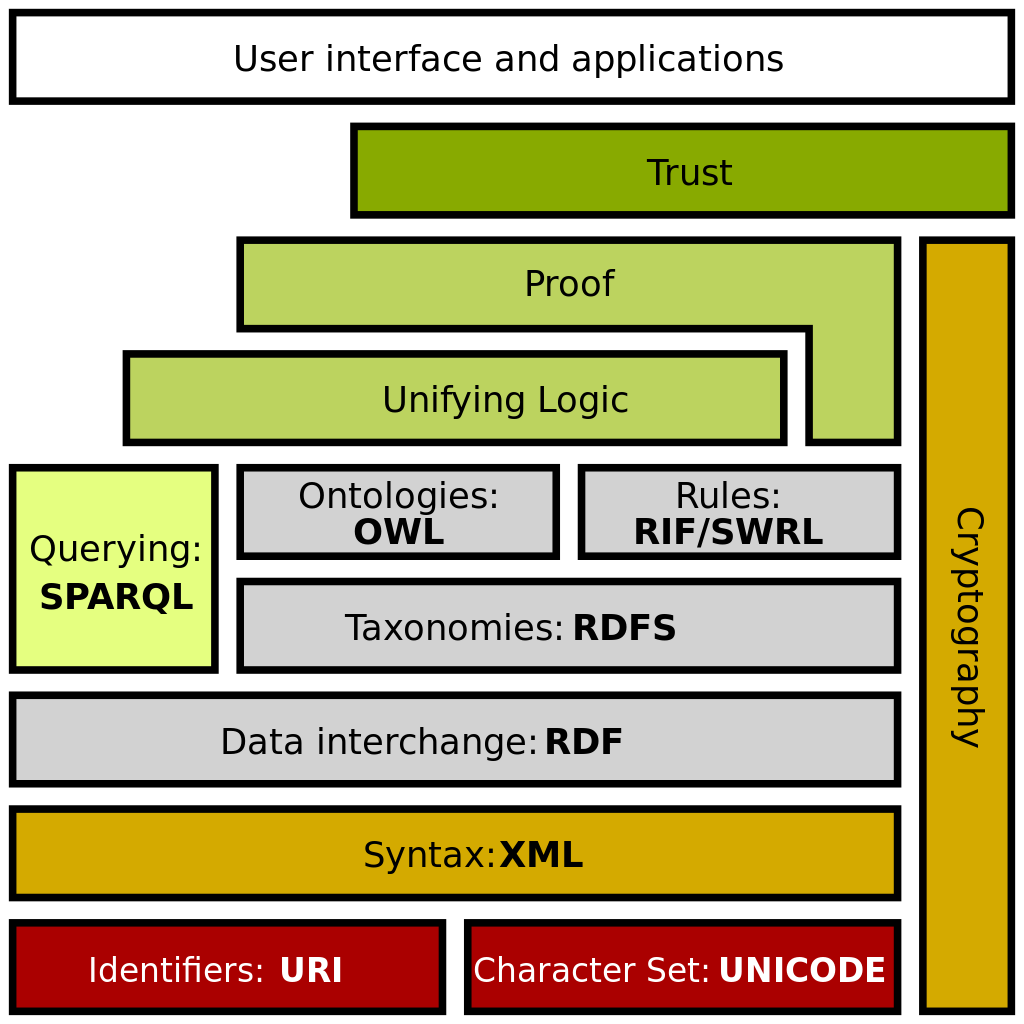
\includegraphics[width=0.8\linewidth]{semantic_web_stack}
    \caption{Arquitectura de la web semántica. Construida en base a múltiples estándares y lenguajes.}
    \label{fig:semantic-web-arq}
\end{figure}

    \subsubsection{Referencias, transporte y principios de los datos enlazados}

El acceso a los datos es fundamental para la arquitectura de la web semántica. Podemos tomar como referencia,
el modelo utilizado por los servidores \textit{Web}, en el cual, los documentos disponibles se encuentran
enlazados a otros de forma descentralizada, esto es, que el documento referenciado no necesariamente se
encuentra en el mismo servidor que está haciendo referencia a él. Estos enlaces, son utilizados por los usuarios
para navegar entre los millones de servidores disponibles en la \textit{Web}.

Las \textit{URI/IRI} y el protocolo \textit{HTTP} son parte fundamental del núcleo que define tanto a la
\textit{World Wide Web} como a la web semántica. En un ejemplo concreto, la \textit{URI}
\url{https://en.wikipedia.org/wiki/Back_to_the_Future} en la \textit{Web}, representa el documento en el
servidor de \textit{wikipedia.org} que contiene información sobre la serie de películas y obras de título
``Volver al Futuro'', en cambio, en el contexto de la web semántica, las \textit{URIs} \url{https://www.wikidata.org/wiki/Q1} representa al
``universo'' como una entidad, la cual es parte del \url{https://www.wikidata.org/wiki/Q3327819} ``multiverso''
y es estudiado por la \url{https://www.wikidata.org/wiki/Q338} ``cosmología''.

Los datos del ejemplo anterior son publicados por \textit{The Wikipedia Fundation} a través del servicio \textit{Wikidata}
\cite{vrandevcic2014wikidata}, pero las relaciones descritas podrían enlazar a otros editores de contenido,
como por ejemplo \textit{DBpedia} \cite{valsecchi2015dbpedia}, el cual es un esfuerzo comunitario para extraer
información estructurada desde distintas fuentes y enlazarlas a través del formato \rdf. Para lograr esto,
los editores de contenido para la web semántica aplican los siguientes principios a sus datos, los cuales
son conocidos como los ``principios para datos enlazados'' o \textit{LinkedData principles} \cite{bizer2011linked}.

\begin{enumerate}
    \item Usar \textit{URIs} como nombres para entidades.
    \item Usar \textit{UIRs HTTP} para que los usuarios puedan buscar y acceder a estas entidades.
    \item Cuando un usuario consulta una \textit{URI}, debes entregar información relevante, utilizando estándares como \rdf y \spql.
    \item Debes incluir enlaces a otras \textit{URIs}, para que los usuarios descubran más entidades.
\end{enumerate}

    \subsubsection{Intercambio de datos}

Los datos de la web semántica son generados por distintas entidades al rededor del mundo, las cuales no estan necesariamente
coordinados entre ellos, por lo que la arquitectura debe soportar la creación distribuida de datos junto con la integración
de multiples fuentes y la interoperabilidad entre los datos creados \cite{bizer2011linked}. Este tipo de requerimientos los
cumplen las estructuras de datos basados en grafos como \rdf. \rdf es un formato basado en la descripción de grafos dirigidos,
los cuales repsentan la información de la forma de tríos \textit{sujeto - predicado - objeto}, en la cual, el \textit{sujeto} y el
\textit{predicado} corresponden a nodos del grafo y el \textit{predicado} es un arco que los relaciona como se puede observar
en la figura \ref{fig:rdf-graph1}. En estos tríos, cualquiera de estos objetos puede tomar el valor de una \textit{URI},
un valor literal (cadenas de texto, numeros o fechas) o simplemente un nodo vacio (identificadores que no pueden ser
referenciados por otra entidad).

\rdf corresponde a la especificación de un lenguaje abstracto para describir relaciones entre entidades, el cual, puede
ser serializado en multiples formatos de texto como \textit{Extensible Markup Language (XML)} \cite{beckett2004rdf} (listing \ref{lst:rdf-xml1})
o en un formato más compacto como \textit{Turtle} \cite{beckett2014rdf} (listing \ref{lst:rdf-turtle}).

\begin{figure*}
    \begin{lstlisting}[language=xml, captionpos=b, caption=Descripción de un documento en \textit{RDF/XML}, label=lst:rdf-xml1, basicstyle=\ttfamily, frame=single]
<rdf:Description rdf:about="http://www.w3.org/TR/rdf-syntax-grammar"
    dc:title="RDF 1.1 XML Syntax">
    <ex:editor>
        <rdf:Description ex:fullName="Dave Beckett">
            <ex:homePage rdf:resource="http://purl.org/net/dajobe/"/>
        </rdf:Description>
    </ex:editor>
</rdf:Description>
    \end{lstlisting}
\end{figure*}

\begin{figure*}
    \begin{lstlisting}[captionpos=b, caption=Descripción de un documento en \textit{RDF/Turtle}, label=lst:rdf-turtle, basicstyle=\ttfamily, frame=single]
@prefix rdf: <http://www.w3.org/1999/02/22-rdf-syntax-ns#> .
@prefix dc: <http://purl.org/dc/elements/1.1/> .
@prefix ex: <http://example.org/stuff/1.0/> .

<http://www.w3.org/TR/rdf-syntax-grammar>
  dc:title "RDF/XML Syntax Specification (Revised)" ;
  ex:editor [
    ex:fullname "Dave Beckett";
    ex:homePage <http://purl.org/net/dajobe/>
  ] .
    \end{lstlisting}
\end{figure*}

%    \subsubsection{Consultas y actualizaciones}
%    \subsubsection{Ontologías y razonamiento}
%    \subsubsection{Reglas}
%    \subsubsection{Seguridad y encriptación}
%    \subsubsection{Unificación e integración}
%    \subsubsection{Confianza}
%    \subsubsection{Aplicaciones}

    \section{Plan de trabajo}

El plan de trabajo descrito en la tabla \ref{tab:plan-trabajo} se basa en el desarrollo
de un prototipo inicial el cual será iterado hasta llegar a una solución final. Ambas etapas
del proyecto deben ser testeadas para evaluar las mejoras realizadas a la base del proyecto
\textit{SPARQLforHumans}.

\begin{table}[h]
    \centering
    \caption{Plan de trabajo para el desarrollo de la memoria propuesta.}
    \label{tab:plan-trabajo}
    \begin{tabular}{|l|l|}
        \hline
        Actividad                                    & Semanas \\ \hline
        Desarrollo del estado del arte               & 2       \\ \hline
        Diseño de la arquitectura de la solución     & 2       \\ \hline
        Programación e implementación de prototipo   & 3       \\ \hline
        Pruebas al rendimiento del prototipo         & 1       \\ \hline
        Programación e implementación de la solución & 7       \\ \hline
        Pruebas al rendimiento de la solución        & 2       \\ \hline
        Desarrollo del informe final                 & 3       \\ \hline
        Correciones                                  & 2       \\ \hline
        Total                                        & 22      \\ \hline
    \end{tabular}
\end{table}


\bibliographystyle{IEEEtran}
\bibliography{IEEEabrv, propuesta.bib}

\newpage

\appendices

\section{Árbol del problema}

\section{Tabla de tiempos SCT}

\begin{table}[h]
    \begin{tabular}{|l|l|}
        \hline
        Actividad                   & Tiempo    \\ \hline
        Planificación               & 2  hrs.    \\ \hline
        Busqueda de información     & 6  hrs.    \\ \hline
        Análisis                    & 2  hrs.    \\ \hline
        Desarrollo                  & 10 hrs.    \\ \hline
        Edición                     & 2  hrs.    \\ \hline
        Video                       & -  hrs.    \\ \hline
        Total                       & -  hrs.    \\ \hline
    \end{tabular}
\end{table}

\section{Enlace al video de la propuesta}

\end{document}
